\documentclass[journal]{IEEEtran}

\usepackage{graphicx}  %needed to include png, eps figures
\usepackage{float}  % used to fix location of images i.e.\begin{figure}[H]

\begin{document}

\title{ECSE 444 - Final Project Initial Report (G21)}

\author{Christopher Ghosn, Qihao Wu, Zichen Gao, Nader Akel}

% make the title area
\maketitle

\section{Concept}
Communication with audio over distances generally takes the form of radios or phones. However, the proliferation of Wi-Fi creates areas where signals do not need to be carried far to go from one device to another. This means that longer-ranged radio signals used in radios and phones are not necessary, keeping those frequencies clear. This requires a pair of devices capable of connecting themselves to a Wi-Fi network so they can transmit audio to each other. 

With the use of two STM32 B-L4S5I-IOT01A Discovery boards, plus peripheral devices such as microphones and speakers, an audio communication link can be established between the two boards over Wi-Fi signals. Voice or audio can be inputted to a microphone, which is transmitted to and compressed within the board using the DFSDM peripheral and CMSIS functions in order to take up less storage and bandwidth. Then, the sending board sends the information over Wi-Fi using the Wi-Fi module to the receiving board, which decompresses the data and emits it through a speaker using the Digital-to-Analog module. As shown in Figure \ref{fig:block} below, the signal processing is a form of compression.

\begin{figure}[H]
    \centering
    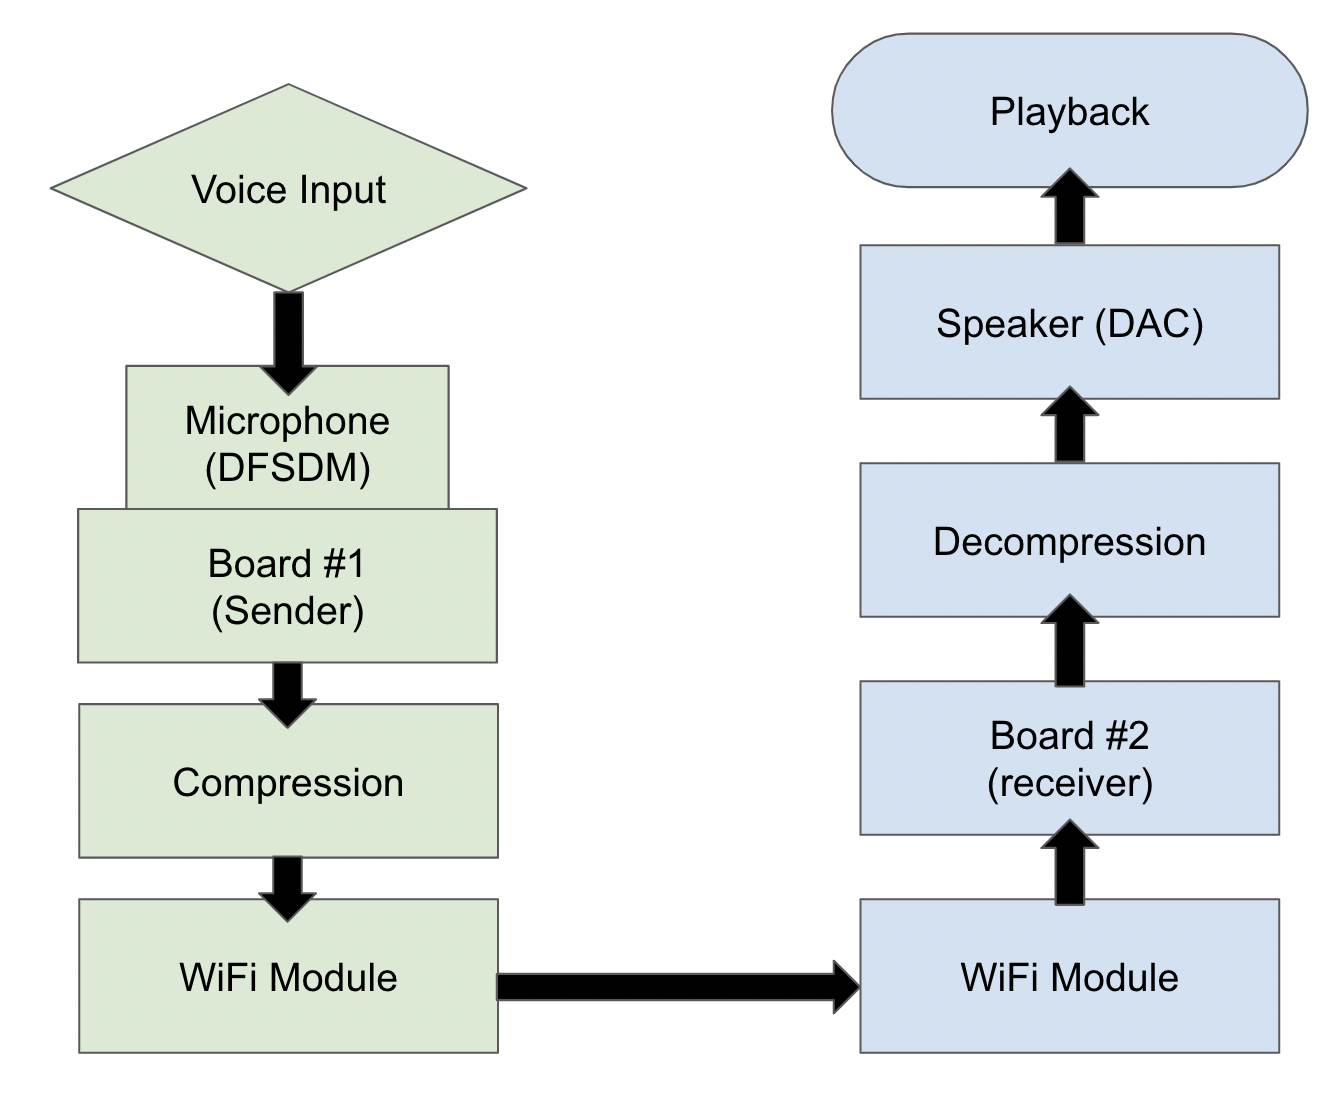
\includegraphics[width=0.9\linewidth]{Screen_Shot_2023-11-17_at_11.38.50_PM.png}
    \caption{Block diagram of system}
    \label{fig:block}
\end{figure}

\section{Subsystems}

\subsection{Audio input and compression}
The audio input and compression (AIC) subsystem takes in raw audio data from DFSDM microphones on the sending board, compresses it using CMSIS functions and formats correctly so that it can be sent over Wi-Fi to the receiving board. Software components of this system include the compression algorithm using CMSIS. Hardware components include the MEMS microphones as well as the DFSDM peripheral, which filters the sound received by the microphones. All hardware components are on the development boards.

On a button press, this subsystem is initiated and the DFSDM microphones start to collect and filter audio data. Using the DMA interface, the function HAL\_DFSDM\_FilterRegularStart\_DMA fills up the buffer, which is 1000 words long, with the word-sized audio samples. An interrupt is raised when the DFSDM has finished collecting data, and the compression algorithm is applied to the filled buffer. After the data is successfully sent to the receiving board, the AIC restarts unless another button press is detected.

This subsystem has not been fully implemented yet. However, we plan on doing more research on methods of audio compression and coming up with an algorithm that makes use of CMSIS functions.

\subsection{Wi-Fi data transfer}
The Wi-Fi data transfer subsystem takes in the compressed data from the AIC subsystem and transfers the data over to the receiving board via Wi-Fi. The software components include code on the receiving and sending boards, which makes use of an existing Wi-Fi library that controls the on-board Wi-Fi module. The hardware components include the Wi-Fi module itself (es-Wifi).

When both the sending and receiving boards are initiated, they connect to an existing Wi-Fi network via credentials (SSID, Password) which are stored in a C header file. Then, servers are created on both boards and the IP address of the receiving board will be printed to a UART terminal. Once connections have been established and the sending board has acquired some audio data, it will use the IP address of the receiving board to send the data via Wi-Fi. The receiving board will send back a message confirming that the data was received, after which the connection is closed.

This subsystem has mostly been implemented. Data transfer between boards has been tested successfully. 

\subsection{Audio decompression and playback}

The audio decompression and playback subsystems take in the data received from the Wi-Fi module on the receiving board and decompresses them using CMSIS functions so it can be played on the speaker. Software components of this system include the decompression algorithm using CMSIS functions. Hardware components include the Digital-to-Analog converter and the speaker. The speaker is a separate hardware component, while the DAC is integrated on the board.

Same as the Audio input and Compression subsystem, this has not been fully implemented yet. 

\section{Evaluation}
We have already tested the Wi-Fi data transfer between the two boards. String of characters were successfully sent to the receiving board. The DAC and Microphone have also been successfully tested simultaneously with the Wi-Fi.
We will be using ITM debugging to evaluate the performance of our code, particularly for the audio compression algorithm. The latency of the WiFi connection will also be assessed by timing the duration between sending a message from one board and receiving a confirmation message back from the other board. We will also use this method to measure the bandwidth of the WiFi connection under different operating conditions by sending huge arrays of values from one board to another and timing the start and confirmation of the completion of the data transfer with ITM debugging.

\section{Progress}

While we currently have a working implementation of a WiFi-based data transfer between two boards, this implementation is written inside of one of the example projects provided for the board by STM32CubeIDE. The lack of an .IOC file makes it much more complicated to configure the pinouts, I/O, and settings of our processor. We are working on finding a way to port the example project into an actual STM32CubeIDE project. Additionally, we are having some issues with memory as our project seems to use more than 70\% of the RAM without any huge arrays being initialized. We believe it may have something to do with the WiFi implementation. 

Since currently have a working implementation of WiFi- based data transfers, audio recording with the DFSDM microphone, and audio playback on the speaker, our next milestone will be to write a very basic version of the walkie talkie software that allows one sender board to record audio of a fixed duration and send it over to another board that will play the audio track on a speaker that is wired to it. After this, we will start adding different features one at a time to the software:
\vspace{10pt}

\begin{itemize}
    \item Audio compression and decompression algorithms to reduce memory usage and WiFi bandwidth requirements

    \item Recording a variable duration for the audio track instead of a fixed one

    \item (Optional) Making a two-way communication between the two boards where messages can both be recorded/sent and received/played on both boards

    \item (Optional) Being able to add more than two boards to the network

    \item (Optional) Using the on-board QSPI flash for increased storage capacity
    
\end{itemize}
\vspace{10pt}

As for performance enhancements to our project, we plan on optimizing the performance of our code through specific compiler directives. We are however also considering doing manual optimization by rewriting some of the HAL or CMSIS functions with our own assembly code to make them faster. The use of SIMD for the audio compression/decompression algorithm is also being considered in order to make it faster as we are working with 8-bit values for audio.

\end{document}